\chapter{Advanced Theorems in Geometry}% by Raiyan Jamil}

\begin{linkb}
   \begin{itemize}
        \item \href{https://www.youtube.com/watch?v=M5XK1DRmvQ4}{Higher theorems Class (Raiyan)}
        \item \href{https://drive.google.com/file/d/1re420K24_RUHWqmKCKolIOnNfHE_DdBx/view}{Class}
        \item \href{https://drive.google.com/file/d/1R0FYTojb1A0fsxsK4U5EbSqYgPjFNQjA/view}{1}, \href{https://drive.google.com/file/d/1jwEP2kMAX0CfU84L9MqnyQi-RkuCPndY/view}{2}, 
			\href{https://drive.google.com/file/d/1Xvko-uY1TfXguyLsI0SJyINVoQ6mLHOB/view}{3},
			\href{https://drive.google.com/file/d/1fm_irN-VGuGjgA4K2xioDTOWrRXyhwHh/view}{4}
			\href{https://drive.google.com/file/d/1j3XsSZXVlacnieq_bEXGKfBtYgxTPMks/view}{5} 
			\href{https://drive.google.com/file/d/11iIS0QZj-Ge798GngpVY1SDxKPipRfIA/view}{6}
			
			\item \href{https://drive.google.com/file/d/1JdYioYeJhqugbqTJBKTQL6XvSNxZh1bw/view}{P Set}
   \end{itemize}
\end{linkb}

Here we are going to learn some advanced theorems in geometry which are mostly belong to Projective Geometry.
\begin{itemize}
	\ii Desargues's Theorem
	\ii Pascal's Theorem
	\ii Pappu's theorem
	\ii Brianchon's Theorem
	\ii Butterfly Theorem
\end{itemize}
%Zhao Notes
\section{Desargues's Theorem}
\begin{theorem}[Desargues's theorem]
$\triangle ABC$ and $\triangle XYZ $ are such that $AB\cap XT = U, BC\cap YZ =V, CA\cap ZX=W$ then, $X,Y, Z$ are collinear if and only if $AX,BY,CZ$ are concurrent.
\end{theorem}

Here we call that $ABC$ and $XYZ$ are perspective from a line if $U,V,W$ are collinear and the line is called the line of perspectivity. 

And if $AX,BY,CZ$ are concurrent then we say, $ABC$ and $XYZ$ are persepctive from a point. 

But, the Desargues's Theorem establishes a realtion between these two perspectivity which is useful in problem solving. 
As, concurrency proof can be given using collinearity.
It is really a very useful theorem. 
\begin{figure}[ht]
\centering
	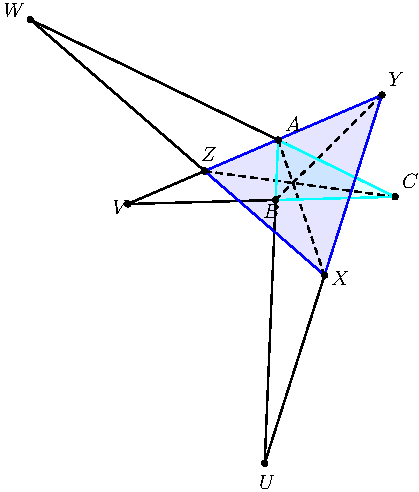
\includegraphics{desargues.pdf}
	\caption{The Desargues' Theorem}
\end{figure}


\section{Pascal's Theorem}
\begin{theorem}[Pascal's Theorem]
If hexagon $ABCDEF$ lies on a circle then $AB\cap DE=X, BC\cap EF =Y, CD\cap FA=Z$ are collinear.
\end{theorem}

\begin{figure}[ht]
\centering
	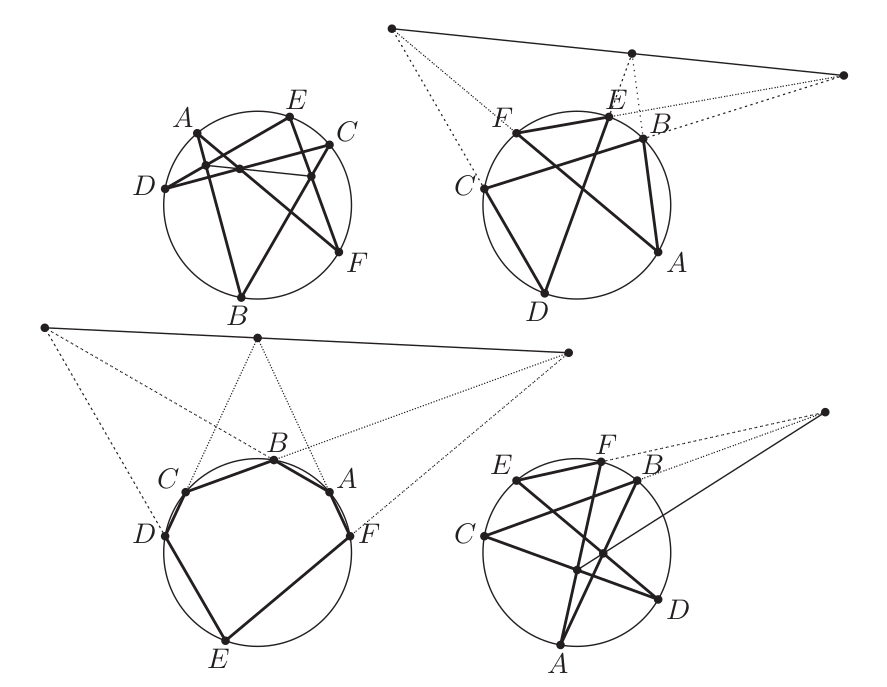
\includegraphics[scale=0.3]{pascals.png}
	\caption{Many Faces of Pascal's Theorem (adapted from Evan Chen's EGMO)}
\end{figure}

\begin{remark*}
If $X,Y,Z$ are collinear then you can not say that $ABCDEF$ lies on a circle.
\end{remark*}
Pascal's Theorem is most useful of these five theorem. It can be applied to as well as triangles, quadrilaterals and pentagons.
Where as an example we apply Pascal's on $AABBCC$ we get $AA\cap BC $ $AB \cap CC$ and $BB \cap CA$ are collinear where $AA$ means the tangent to the circumcircle at $A$, and so on.

So, it seems very useful in different problems containing triangles, quadrilaterals, pentagons and hexagons.


\section{Pappu's theorem}
\begin{theorem}[Pappu's Theorem]
$A,B,C,D,E,F$ are six poins on the plane. Let $AB\cap DE=X, BC\cap EF =Y, CD\cap FA=Z$. Then, $A,C,E$ and $B,D,F$ are collinear if and only if $X,Y,Z$ are collinear.
\end{theorem}
You may wonder that, Problem 2 of IMO 2019 can be solved using Pappu's Theorem along with some other facts.
\begin{figure}[ht]
\centering
	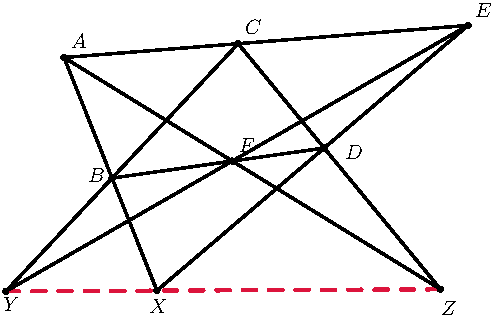
\includegraphics{pappu.pdf}
	\caption{Pappu's Theorem}
\end{figure}

\section{Brianchon's Theorem}
\begin{theorem}[Brianchon's Theorem]
$ABCDEF$ is a tangential hexagon (i.e. Sides of the hexagon are externally tangent to a common circle). Then, $AD,BE,CF$ are concurrent.
\end{theorem}
Brianchon's Theorem can be derived directly from Pascal's Theorem by only interchanging the words 'points' and 'line', and making whatever
grammatical adjustments that are necessary.

Brianchon's and Pascal's theorem form Pole Polar duality of Projective Geometry. 
\begin{figure}[ht]
\centering
	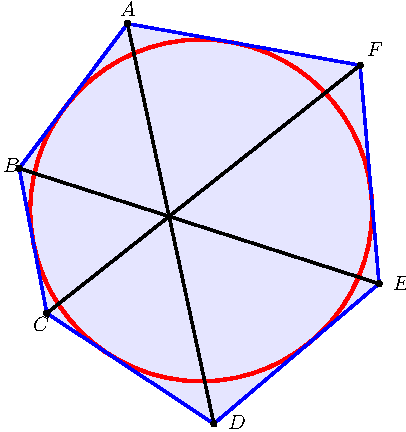
\includegraphics{brianchon.pdf}
	\caption{Brianchon's Theorem}
\end{figure}
Point to be noted that, we can take $C,D,E$ collinear, then the polygon becomes a pentagon. We also can take $A,B,C$ and $D,E,F$ collinear, then the polygon becomes a tangential quadrilateral.
Here, $B,E$ become point of tangency. Let, $CD$ and $FA$ touches the circle at $G,H$ then, $AD,CF,BE,GH$ all are concurrent.

\begin{figure}[htt]
\centering
	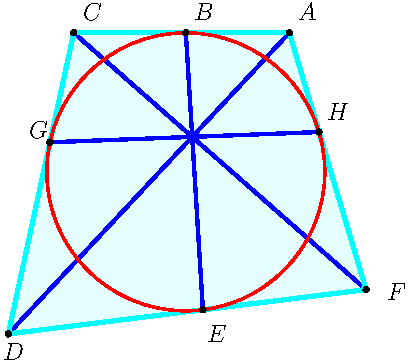
\includegraphics[scale=1]{brian-quad.pdf}
	\caption{Brianchon's Theorem on a quadrilateral.}
\end{figure}

\section{Butterfly Theorem}
\begin{theorem}[Butterfly Theorem]
$AB$ be a chord of a circle with midpoint $M$. Let two chords through $M$ of the circle are $CD$ and $EF$. $CE\cap AB=X$ and $DF\cap AB=Y$. Then, $MX=MY$. 
\end{theorem}
%The converse is also true for Butterfly Theorem. If $
\begin{figure}[ht]
\centering
	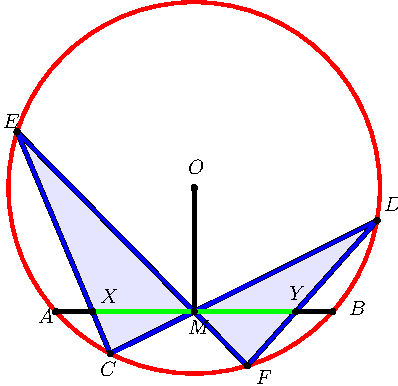
\includegraphics{butterfly.pdf}
	\caption{The butterfly theorem, look polygon $CEFD$ looks like a butterfly!}
\end{figure}


The Theorem is also tru if the chord is not a chord of the circle i.e. the line lies outside the circle, as the next theorem says.




\begin{theorem}[Extended Butterfly Theorem]
Let $\ell$ be a line on the plane of a circle $\omega$. $O$ is the center of the circle. Let $M$ be a point on $\ell$ such that $OM\perp \ell$. Let two lines through $M$ intersects the circle at $C,E$ and $D,F$ respectively. Let $DE$ and $CF$ meet $\ell$ at $B,A$ respectively. And $CD$ and $EF$ meet $\ell$ at $H,G$ respectively. Now, $AM=BM$ and $GM=HM$.
%----------
%$AB$ be a chord of a circle with midpoint $M$. Let two chords through $M$ of the circle are $CD$ and $EF$. $CE\cap AB=X$ and $DF\cap AB=Y$. Then, $MX=MY$. 
\end{theorem}

\begin{figure}[ht]
\centering
	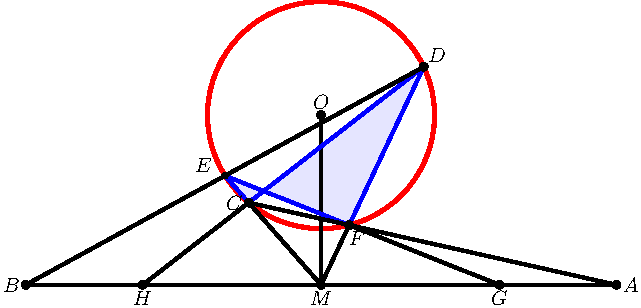
\includegraphics{butterfly-extended.pdf}
	\caption{Extended Butterfly Theorem}
\end{figure}

\section{Practise Problems}


\begin{problem}


	\begin{hint}
	\addhint{}
	\addhint{}
	\end{hint}
\end{problem}

\begin{problem}


	\begin{hint}
	\addhint{}
	\addhint{}
	\end{hint}
\end{problem}

\begin{problem}


	\begin{hint}
	\addhint{}
	\addhint{}
	\end{hint}
\end{problem}

\begin{problem}


	\begin{hint}
	\addhint{}
	\addhint{}
	\end{hint}
\end{problem}

\begin{problem}


	\begin{hint}
	\addhint{}
	\addhint{}
	\end{hint}
\end{problem}

\begin{problem}


	\begin{hint}
	\addhint{}
	\addhint{}
	\end{hint}
\end{problem}

\begin{problem}


	\begin{hint}
	\addhint{}
	\addhint{}
	\end{hint}
\end{problem}